\section{Applications}
We present some case studies that apply the gradient estimators to implicit models. Detailed settings (architecture, learning rate, etc.) are presented in Appendix \ref{sec:appendix_stein}. Implementation is released at \url{https://github.com/YingzhenLi/SteinGrad}.

\subsection{Synthetic example: Hamiltonian flow with approximate gradients}
We first consider a simple synthetic example to demonstrate the accuracy of the proposed gradient estimator. More precisely we consider the kernel induced Hamiltonian flow (\emph{not} an exact sampler) \citep{strathmann:kmc2015} on a 2-dimensional banana-shaped object: $\x \sim \mathcal{B}(\x; b=0.03, v=100) \Leftrightarrow  x_1 \sim \mathcal{N}(x_1; 0, v), x_2 = \epsilon + b(x_1^2 - v), \epsilon \sim \mathcal{N}(\epsilon; 0, 1)$. The approximate Hamiltonian flow is constructed using the same operator as in Hamiltonian Monte Carlo (HMC) \citep{duane:hmc1987, neal:mcmc2011}, except that the exact score function $\nabla_{\x} \log \mathcal{B}(\x)$ is replaced by the approximate gradients. We still use the exact target density to compute the rejection step as we mainly focus on testing the accuracy of the gradient estimators. We test both versions of the predictive Stein gradient estimator (see Section \ref{sec:predictive_estimator}) since we require the particles of parallel chains to be independent with each other. 
%
We fit the gradient estimators on $K=200$ training datapoints from the target density. The bandwidth of the RBF kernel is computed by the median heuristic and scaled up by a scalar between $[1, 5]$. All three methods are simulated for $T=2,000$ iterations, they share the same initial locations that are constructed by target distribution samples plus Gaussian noises of standard deviation 2.0, and the results are averaged over 200 parallel chains. 

We visualise the samples and some MCMC statistics in Figure \ref{fig:banana_example}. 
%
In general all the resulting Hamiltonian flows
are HMC-like, which give us the confidence that the gradient estimators extrapolate reasonably well at unseen locations that are close to the training data. However all of these methods have trouble exploring the extremes, because at those locations there are very few or even no training data-points. Indeed we found it necessary to use large (but not too large) bandwidths, in order to both allow exploration of those extremes, and ensure that the corresponding test function is not too smooth. In terms of quantitative metrics, the acceptance rates are reasonably high for all the gradient estimators, and the KSD estimates (across chains) as a measure of sample quality are also close to that computed on HMC samples. The returned estimates of $\mathbb{E}[x_1]$ are close to zero which is the ground true value. We found that the non-parametric Stein gradient estimator is more sensitive to hyper-parameters of the dynamics, e.g.~the stepsize of each HMC step.
%
We believe a careful selection of the kernel (e.g.~those with long tails) and a better search
for the hyper-parameters (for both the kernel and the dynamics) can further improve the
sample quality and the chain mixing time, but this is not investigated here.

\begin{figure}[t]
\vspace{-0.15in}
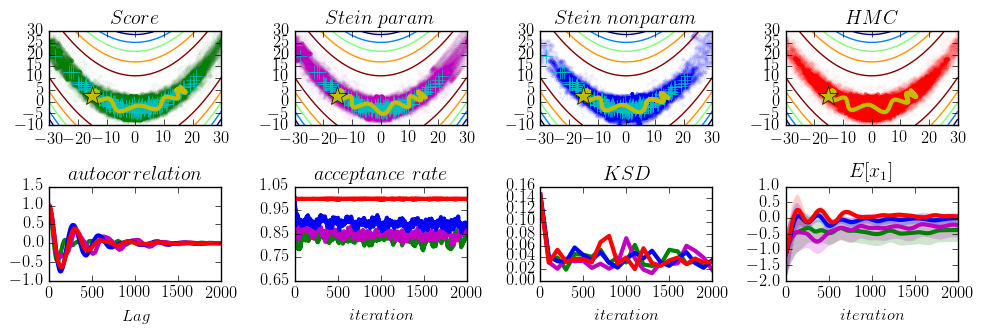
\includegraphics[width=1.0\linewidth]{figs/banana.png}
\vspace{-0.2in}
\caption{Kernel induced Hamiltonian flow compared with HMC. Top: samples generated from the dynamics, training data (in cyan), an the trajectory of a particle for $T=1$ to $200$ starting at the star location (in yellow). Bottom: statistics computed during simulations. See main text for details.}
\vspace{-0.1in}
\label{fig:banana_example}
\end{figure}

\subsection{Meta-learning of approximate posterior samplers for Bayesian NNs}
\label{sec:chap6_meta}
%
One of the recent focuses on meta-learning has been on learning optimisers for training deep neural networks, e.g.~see \cite{andrychowicz:gradient2016, li:optimize2016}. Could analogous goals be achieved for approximate inference? In this section we attempt to learn an approximate posterior sampler for Bayesian neural networks (Bayesian NNs, BNNs) that generalises to \emph{unseen} datasets and architectures, and we refer to Section \ref{sec:chap5_wild_applications} for a motivation of this approach. 

In a nutshell, we consider a binary classification task: $p(y = 1|\x, \mparam) = \text{sigmoid}(\text{NN}_{\mparam}(\x))$, $p_0(\mparam) = \mathcal{N}(\mparam; \bm{0}, \mathbf{I})$. After observing the training data $\data = \{(\x_n, y_n)\}_{n=1}^N$, we first obtain the approximate posterior $q_{\vparam}(\mparam) \approx p(\mparam | \data) \propto p_0(\mparam) \prod_{n=1}^N p(y_n | \x_n, \mparam)$, then approximate the predictive distribution for a new observation as $ p(y^*=1|\x^*, \data) \approx \frac{1}{K} \sum_{k=1}^K p(y^*=1|\x^*, \mparam^k), \mparam^k \sim q_{\vparam}(\mparam). $ 
%
In this task we define an implicit approximate posterior distribution $q_{\vparam}(\mparam)$ as the following \emph{stochastic} RNN $\mparam_{t+1} = \f(\mparam_t, \nabla_t, \bm{\epsilon}_t)$: given the current location $\mparam_t$ and the mini-batch data $\{ (\x_m, y_m) \}_{m=1}^M$, the update for the next step is
\begin{equation}
\begin{aligned}
\mparam_{t+1} &= \mparam_{t} + \zeta \Delta_{\vparam}(\mparam_t, \nabla_t) + \bm{\sigma}_{\vparam}(\mparam_t, \nabla_t) \odot \bm{\epsilon}_t, \quad \bm{\epsilon}_t \sim  \mathcal{N}(\bm{\epsilon}; \bm{0}, \mathbf{I}),\\
\nabla_t &= \nabla_{\mparam_t} \left[ \frac{N}{M} \sum_{m=1}^M \log p(y_m|\x_m, \mparam_t) + \log p_0(\mparam_t) \right] .
\end{aligned}
\end{equation}
The coordinates of the noise standard deviation $\bm{\sigma}_{\vparam}(\mparam_t, \nabla_t)$ and the moving direction $\Delta_{\vparam}(\mparam_t, \nabla_t)$ are parametrised by a \emph{coordinate-wise} neural network, i.e.~
$$\bm{\sigma}_{\vparam}(\mparam_t, \nabla_t) = [\bm{\sigma}_{\vparam}(\mparam_t(1), \nabla_t(1)), ..., \bm{\sigma}_{\vparam}(\mparam_t(d), \nabla_t(d)) ]^{\text{T}}$$
with $\mparam_t(i)$ denoting the $i^{\text{th}}$ dimension of vector $\mparam_t$ (similarly for $\nabla_t(i)$ and $\Delta_{\vparam}(\mparam_t, \nabla_t)$).
%
If properly trained, this neural network will learn the best combination of the current location and gradient information, and produce approximate posterior samples efficiently on different probabilistic modelling tasks.

We propose using the variational inference objective (\ref{eq:vi_objective_entropy}) computed on the samples $\{ \mparam_t^k \}$ to learn the variational parameters $\vparam$. 
%
More specifically, we simulate the approximate sampler for $T = 10$ transitions and sum over the variational lower-bounds computed on the samples of every step. This gives the maximisation objective
$$\mathcal{L}(\vparam) = \sum_{t=1}^T \mathcal{L}_{\text{VI}}(q_t),$$
with $q_t(\mparam)$ as the marginal distribution of $\mparam_t$ (therefore depends on $\vparam$). In practice the variational lower-bound $\mathcal{L}_{\text{VI}}(q_t)$ is further approximated by Monte Carlo and data sub-sampling:
$$ \mathcal{L}_{\text{VI}}(q_t) \approx \frac{N}{K M} \sum_{m = 1}^M \sum_{k=1}^K \log p(y_m|\x_m, \mparam_t^k) + \log p_0(\mparam_t^k) - \log q_t(\mparam_t^k).$$
%
Since in this case the gradient of the log joint distribution can be computed analytically, we only approximate the gradient of the entropy term $\mathbb{H}[q]$ as in (\ref{eq:entropy_gradient}), with the exact score function replaced by the presented gradient estimators. 

\begin{figure}[t]
\subfigure[SGLD]{
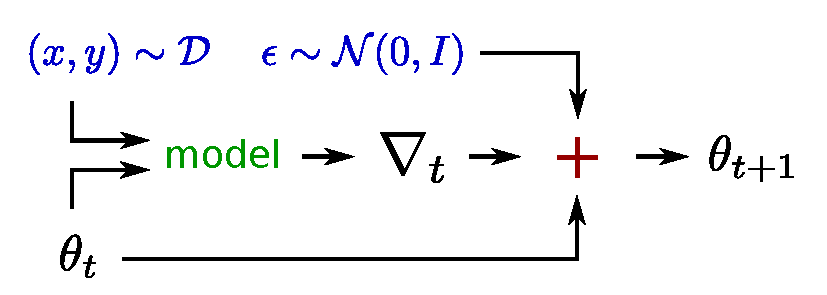
\includegraphics[width=0.45\linewidth]{figs/sgld_sampler.pdf}}
\hfill
\subfigure[NN-based approx.~sampler]{
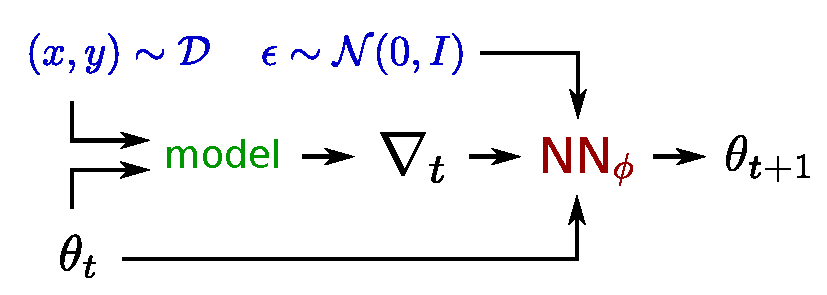
\includegraphics[width=0.45\linewidth]{figs/nn_sampler.pdf}}
\caption{Comparing the computation graphs of the two samplers. SGLD can be viewed as stochastic gradient descent plus properly scaled Gaussian noise. Instead of using the ``plus'' operation, the NN-based sampler combine the three inputs with a neural network, and the parameters $\vparam$ are then trained by the method described in the main text.}
\label{fig:sgld_nn_sampler_compare}
\end{figure}

We briefly describe the test protocol. We take from the UCI repository \citep{Lichman:uci_data2013} six binary classification datasets (australian, breast, crabs, ionosphere, pima, sonar), train an approximate sampler on crabs with a small neural network that has one 20-unit hidden layer with \emph{ReLU} activation, and generalise to the remaining datasets with a bigger network that has 50 hidden units and uses \emph{sigmoid} activation. We use ionosphere as the validation set to tune $\zeta$. The remaining 4 datasets are further split into 40\% training subset for simulating samples from the approximate sampler, and 60\% test subsets for evaluating the sampler's performance.
%
Besides the gradient estimators we also compare with two baselines: an approximate posterior sampler trained by maximum a posteriori (MAP), and stochastic gradient Langevin dynamics (SGLD) \citep{welling:sgld2011} evaluated on the test datasets directly. A comparison between SGLD and the proposed neural network based approximate sampler is visualised in Figure \ref{fig:sgld_nn_sampler_compare}. 

For architecture details, we use a one hidden layer neural network with 20 hidden units to compute the noise standard deviation $\bm{\sigma}_{\vparam}(\mparam_t, \nabla_t)$ and the moving direction $\Delta_{\vparam}(\mparam_t, \nabla_t)$ of the next update. Softplus non-linearity is used for the hidden layer and to compute the noise variance we apply ReLU activation to ensure non-negativity. The step-size $\zeta$ is selected as $10^{-5}$ which is tuned on the KDE approach. For SGLD step-size $10^{-5}$ also returns overall good results.\footnote{We note here that the results can be further improved with carefully tuned learning rate for both SGLD and the NN-based samplers, but here we are mainly interested in the same step-size set-up in order to compare the velocity of the particles defined by the underlying dynamics of the samplers.}
We report the results using the non-parametric Stein gradient estimator as we found it works better than the parametric version. The RBF kernel is applied for gradient estimation, with the hyper-parameters determined by a grid search on the bandwidth $\sigma^2 \in \{0.25, 1.0, 4.0, 10.0, \text{median trick} \}$ and $\eta \in \{0.1, 0.5, 1.0, 2.0\}$.

\begin{figure}[t]
\centering
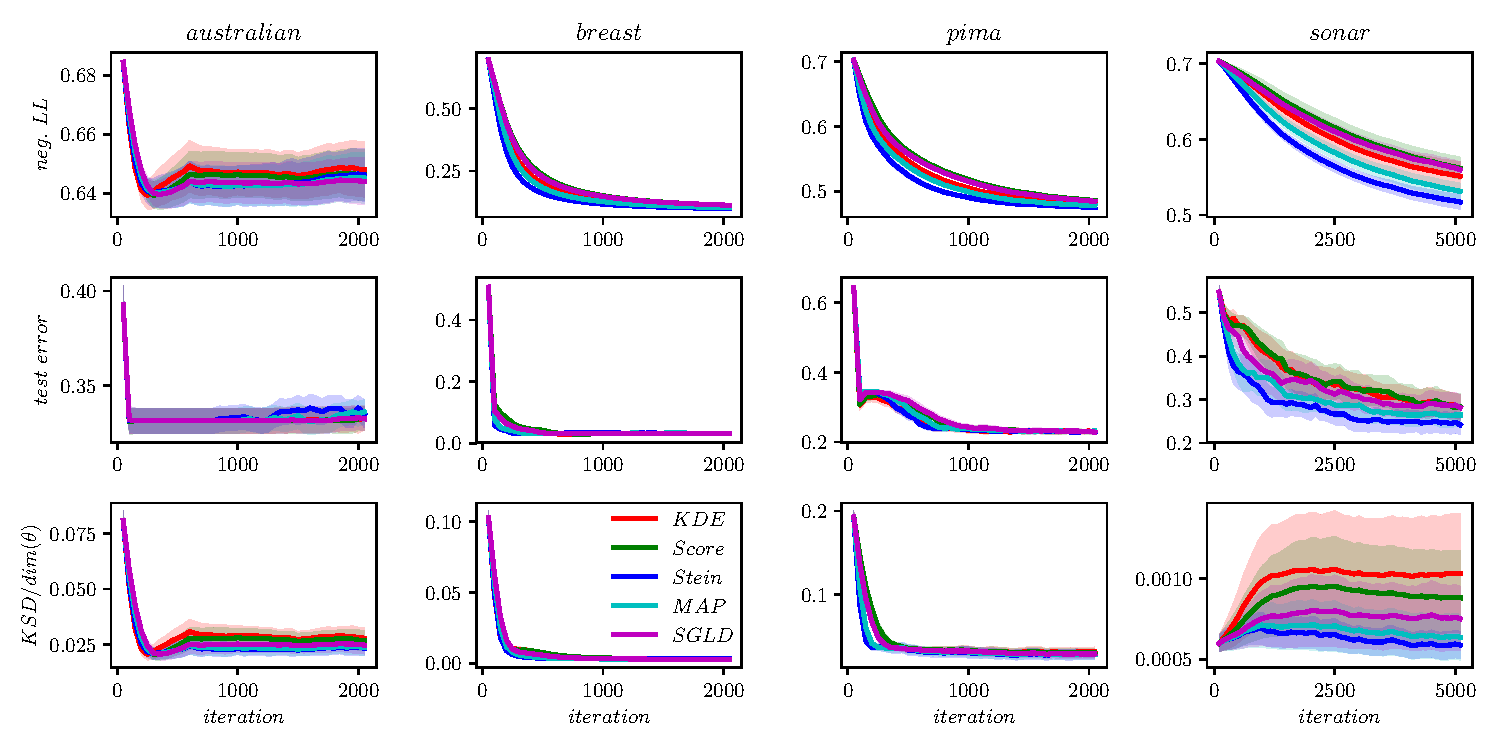
\includegraphics[width=1.0\linewidth]{figs/nn_sampler_results_new.pdf}
\vspace{-0.2in}
\caption{Generalisation performances for trained approximate posterior samplers.}
\vspace{-0.1in}
\label{fig:nn_sampler_results}
\end{figure}

Figure \ref{fig:nn_sampler_results} presents the (negative) test log-likelihood (LL), classification error, and an estimate of the KSD U-statistic $\mathcal{S}^2_U(p(\mparam | \D), q(\mparam))$ (with data sub-sampling) over 5 splits of each test dataset.\footnote{After conference publication (see publication page) I fixed a few issues of the previous implementation (mainly for the score matching estimator) and re-run the experiments, which is reported in this thesis.} 
%
The Stein approach performs equally well or a little better than SGLD in terms of test-LL and test error. The KDE method is slightly worse and is close to MAP, indicating that the KDE estimator does not provide a very informative gradient for the entropy term.
%
%The MAP model under-performs for test log-likelihood and KSD metrics, presumably because the noise variance $\bm{\sigma}$ has been turned off during learning thus having discovered an optimiser instead. 
%
The score matching estimator method produces the worst results among the trained samplers even after carefully tuning the bandwidth and the regularisation parameter $\eta$, although the difference is not significant. 
%
Future work should investigate the usage of advanced recurrent neural networks such as an LSTM \citep{hochreiter:lstm1997}, which is expected to return better performance.

\subsection{Towards addressing mode collapse in GANs using entropy regularisation}
GANs are notoriously difficult to train in practice. Besides the instability of gradient-based minimax optimisation which has been partially addressed by many recent proposals \citep{salimans:training2016, arjovsky:wgan2017, berthelot:began2017}, they also suffer from mode collapse. We propose adding an entropy regulariser to the GAN generator loss. Concretely, assume the generative model $p_{\mparam}(\x)$ is implicitly defined by $\x = \f_{\bm{\theta}}(\z), \z \sim p_0(\z)$, then the generator's loss is defined by 
\begin{equation}
\tilde{\mathcal{J}}_{\text{gen}}(\mparam) = \mathcal{J}_{\text{gen}}(\mparam) - \alpha \mathbb{H}[p_{\mparam}(\x)],
\label{eq:gan_regularised_general}
\end{equation}
where $\mathcal{J}_{\text{gen}}(\mparam)$ is the original loss function for the generator from any GAN algorithm and $\alpha$ is a hyper-parameter. In practice the gradient of (\ref{eq:gan_regularised_general}) is estimated using Monte Carlo.

As an illustrating example, in the following we consider the very recently proposed boundary equilibrium GAN (BEGAN) \citep{berthelot:began2017} approach. In BEGAN the discriminator is defined as an auto-encoder $D_{\hparam}(\x)$ that reconstructs the input $\x$. After selecting a ratio parameter $\gamma > 0$, a control rate $\beta_0$ initialised at 0, and a ``learning rate'' $\lambda > 0$ for the control rate, the loss functions for the generator $\x = \f_{\mparam}(\z), \z \sim p_0(\z)$ and the discriminator are:
\begin{equation}
\begin{aligned}
& \mathcal{J}(\x) =  || D_{\hparam}(\x) - \x ||, \quad || \cdot || = || \cdot ||_2^2 \text{ or } || \cdot ||_1, \\
& \mathcal{J}_{\text{gen}}(\mparam; \hparam) = \mathcal{J}(\f_{\mparam}(\z)), \quad \z \sim p_0(\z)  \\ 
& \mathcal{J}_{\text{dis}}(\hparam; \mparam) = \mathcal{J}(\x) - \beta_t \mathcal{J}_{\text{gen}}(\mparam; \hparam), \quad \x \sim \D \\
& \beta_{t+1} = \beta_t + \lambda (\gamma \mathcal{J}(\x) - \mathcal{J}(\f_{\mparam}(\z))).
\end{aligned}
\label{eq:began_original}
\end{equation}
The main idea behind BEGAN is that, as the reconstruction loss $\mathcal{J}(\cdot)$ is approximately Gaussian distributed, with $\gamma = 1$ the discriminator loss $\mathcal{J}_{\text{dis}}$ is (approximately) proportional to the Wasserstein distance between loss distributions induced by the data distribution $p_{\D}(\x)$ and the generator $p(\x)$. In practice it is beneficial to maintain the equilibrium $\gamma \mathbb{E}_{p_{\D}} \left[ \mathcal{J}(\x) \right] = \mathbb{E}_{p} \left[ \mathcal{J}(\x) \right] $ through the optimisation procedure described in (\ref{eq:began_original}) that is motivated by proportional control theory. This approach effectively stabilises training, however it suffers from catastrophic mode collapse problem (see the left most panel in Figure \ref{fig:gan_samples}). 

We empirically investigate the entropy regularisation idea on BEGAN using (continuous) MNIST. 
As described before, we simply subtract an entropy term from the generator's loss function, i.e. with $K$ samples $\z^1, ..., \z^k \sim p_0(\z)$,
\begin{equation}
\tilde{\mathcal{J}}_{\text{gen}}(\mparam; \hparam) = \frac{1}{K} \sum_{k=1}^K \mathcal{J}(\f_{\mparam}(\z^k)) + \alpha \frac{1}{K} \sum_{k=1}^K \log p(\f_{\mparam}(\z^k)),
\end{equation}
where the rest of the optimisation objectives remains as in (\ref{eq:began_original}). This procedure would maintain the equilibrium $\gamma \mathbb{E}_{p_{\D}} \left[ \mathcal{J}(\x) \right] = \mathbb{E}_{p} \left[ \mathcal{J}(\x) \right] - \alpha \mathbb{H}[p]$. We approximate the gradient $\nabla_{\mparam} \mathbb{H}[p]$ using the estimators presented above. For the purpose of updating the control rate $\beta_t$ two strategies are considered to approximate the contribution of the entropy term. The first proposal considers a plug-in estimate of the entropy term with a KDE estimate of $p(\x)$, which is consistent with the KDE estimator but not necessary with the other two (as they use kernels when representing $\log p(\x)$ or $\nabla_{\x} \log p(\x)$). The second one uses a proxy of the entropy loss $-\tilde{\mathbb{H}}[p] = \frac{1}{K} \sum_{k=1}^K \nabla_{\x^k} \log \hat{p}(\x^k)^{\text{T}} \x^k$ with $\nabla_{\x^k} \log \hat{p}(\x^k)$ is the approximate gradient obtained by the estimators. It is the surrogate loss used to (approximately) compute $\nabla_{\vparam} \mathbb{H}[p]$:
$$
\nabla_{\vparam} \mathbb{H}[p] \approx \nabla_{\vparam} \tilde{\mathbb{H}}[p] = \frac{1}{K} \sum_{k=1}^K \nabla_{\x^k} \log \hat{p}(\x^k)^{\text{T}} \nabla_{\vparam} \x^k.
$$

We compare the non-parametric V-statistic Stein gradient estimator to both KDE and score matching estimators. We use a convolutional generative network and a convolutional auto-encoder and select the hyper-parameters of BEGAN $\gamma \in \{0.3, 0.5, 0.7\}$, $\alpha \in [0, 1]$ and $\lambda = 0.001$. The Epanechnikov kernel $\mathcal{K}(\x, \x') := \frac{1}{d} \sum_{j=1}^d (1 - (x_j - x'_j)^2)$ is used as the pixel values lie in a unit interval (see Appendix \ref{sec:appendix_stein} for the expression of the score matching estimator), and to ensure the boundary condition we clip the pixel values into range $[10^{-8}, 1-10^{-8}]$. Readers are referred to Appendix \ref{sec:appendix_stein} for a detailed experimental set-up.

The generated images are visualised in Figure \ref{fig:gan_samples}. BEGAN without entropy regularisation fails to generate diverse samples even when trained with learning rate decay. The other three images clearly demonstrate the benefit of the entropy regularisation technique, with the Stein approach obtaining the highest diversity without compromising visual quality.

%
We further consider four metrics to assess the trained models quantitatively. First 500 samples are generated for each trained model, then we compute their nearest neighbours in the training set using $\ell_1$ distance, and obtain a probability vector $\mathbf{p}$ by averaging over these neighbour images' label vectors. In Figure \ref{fig:gan_results} we depict the entropy of $\mathbf{p}$  (top left), averaged $\ell_1$ distances to the nearest neighbour (top right), and the difference between the largest and smallest elements in $\mathbf{p}$ (bottom right). The error bars are obtained by 5 independent runs. These results demonstrate that the Stein approach performs significantly better than the other two, in that  it learns a better generative model not only faster but also in a more stable way. Interestingly the KDE approach achieves the lowest average $\ell_1$ distance to nearest neighbours, possibly because it tends to memorise training examples. We next train a fully connected network $\pi(\y|\x)$ on MNIST that achieves 98.16\% text accuracy, and compute on the generated images an empirical estimate of the inception score \citep{salimans:training2016} $\mathbb{E}_{p(\x)}[\mathrm{KL}[\pi(\y|\x) || \pi(\y)] ]$ with $\pi(\y) = \mathbb{E}_{p(\x)}[\pi(\y|\x)]$ (bottom left panel). High inception score indicates that the generate images tend to be both realistic looking and diverse, and again the Stein approach out-performs the others on this metric by a large margin. 

Concerning computation speed, all the three methods are of the same order: 10.20s/epoch for KDE, 10.85s/epoch for Score, and 10.30s/epoch for Stein.\footnote{All the methods are timed on a machine with an NVIDIA GeForce GTX TITAN X GPU.} This is because $K < d$ (in the experiments $K=100$ and $d=784$) so that the complexity terms are dominated by kernel computations ($\mathcal{O}(K^2 d)$) required by all the three methods. Also for a comparison, the original BEGAN method without entropy regularisation runs for 9.05s/epoch. Therefore the main computation cost is dominated by the optimisation of the discriminator/generator, and the proposed entropy regularisation can be applied to many GAN frameworks with little computational burden.

\begin{figure}[t]
\vspace{-0.2in}
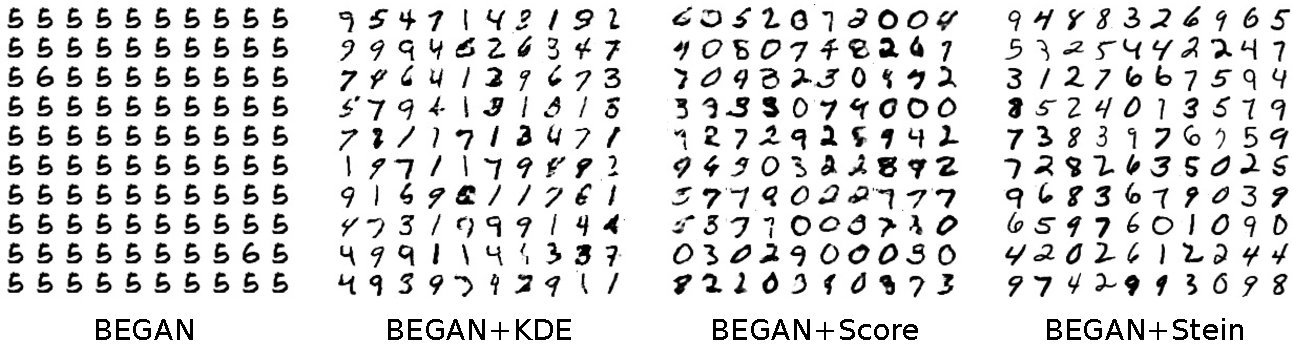
\includegraphics[width=1.0\linewidth]{figs/gan_samples.pdf}
\vspace{-0.2in}
\caption{Visualisation of generated images from trained BEGAN models.}
\label{fig:gan_samples}
\vspace{0.1in}
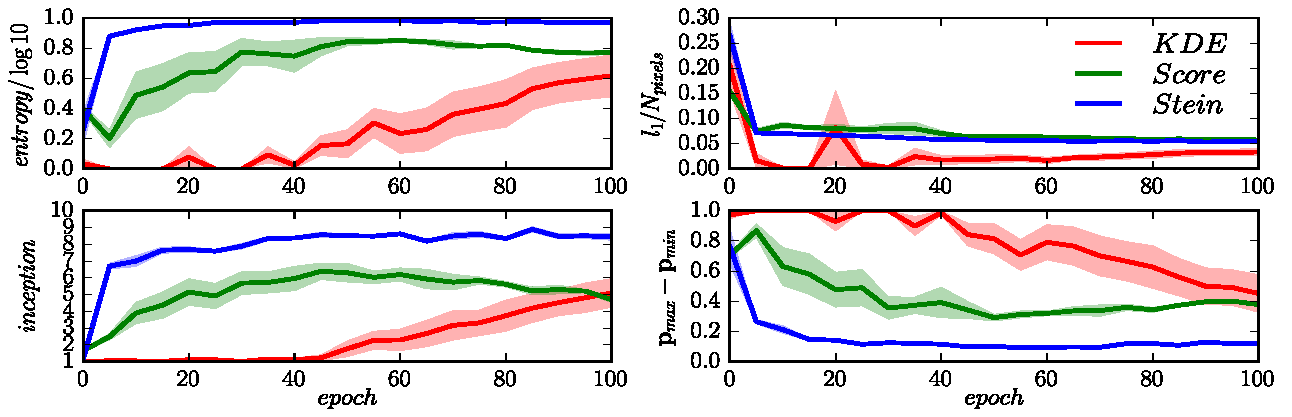
\includegraphics[width=1.0\linewidth]{figs/gan_results.pdf}
\vspace{-0.2in}
\caption{Quantitative evaluation on entropy regularised BEGAN. The higher the better for the LHS panels and the other way around for the RHS ones. See main text for details.}
\vspace{-0.1in}
\label{fig:gan_results}
\end{figure}
